\section{Best views estimation}\label{sec:best-views-estimation}

The estimation of the best views for a constellation of sensors requires the ability to generate accurate sensor data for each type of sensor and also an efficient approach to compute the surface coverage area that we are trying to maximize. The next sections explain how the sensor data is analyzed and also present the approaches used to estimate the best constellation of sensors for a given simulation world.

\subsection{Reference surface point cloud}

The first step in the processing pipeline includes the generation of the multiple object reference point cloud that is built by transforming the point cloud associated with the target \gls{cad} model into each target object instance within the simulation world (example shown in \cref{fig:reference-cloud}), followed by the merge of each object instance point cloud into a single point cloud in the world coordinate system, which later on is filtered with a voxel grid algorithm in order to perform a regular space partition and extract the surface voxels centroids that contain points. This approach allows to generate a reference point cloud with a constant surface point density, which will be critical later on when computing the surface coverage area percentage achieved with a given sensor constellation.

%\begin{algorithm}
%	\caption{Generation of the reference point cloud}
%	\label{alg:reference-pointcloud}
%	\begin{algorithmic}[1]
%		\State \textbf{Input:}
%		\State $P \gets$ CAD model point cloud
%		\State $N \gets$ target objects simulation names
%		\State $F \gets$ cell size for the voxel grid filter
%		\Procedure{ReferencePointCloud}{$P,N,F$}
%			\State $r \gets Empty$\Comment{merged point cloud}
%			\ForAll{n names in N}
%				\State $w \gets GetModelWorldPose(n)$
%				\State $p \gets TransformPointCloud(P,w)$
%				\State $r \gets Merge(r,p)$
%			\EndFor
%			\State $r \gets FilterWithVoxelGrid(r,F)$
%			\State \textbf{return} $(r)$
%		\EndProcedure
%	\end{algorithmic}
%\end{algorithm}

\begin{figure}
	\centering
	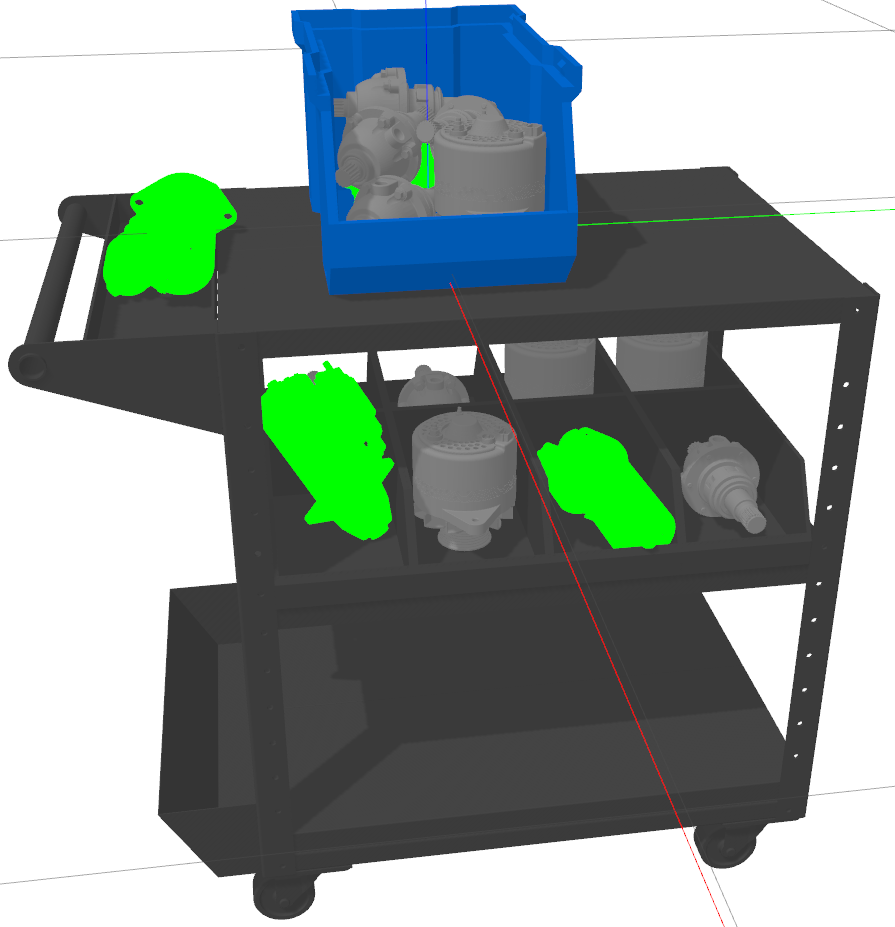
\includegraphics[height=.15\textheight]{sensor-data-processing/multimodel-environment}\hspace{1em}
%	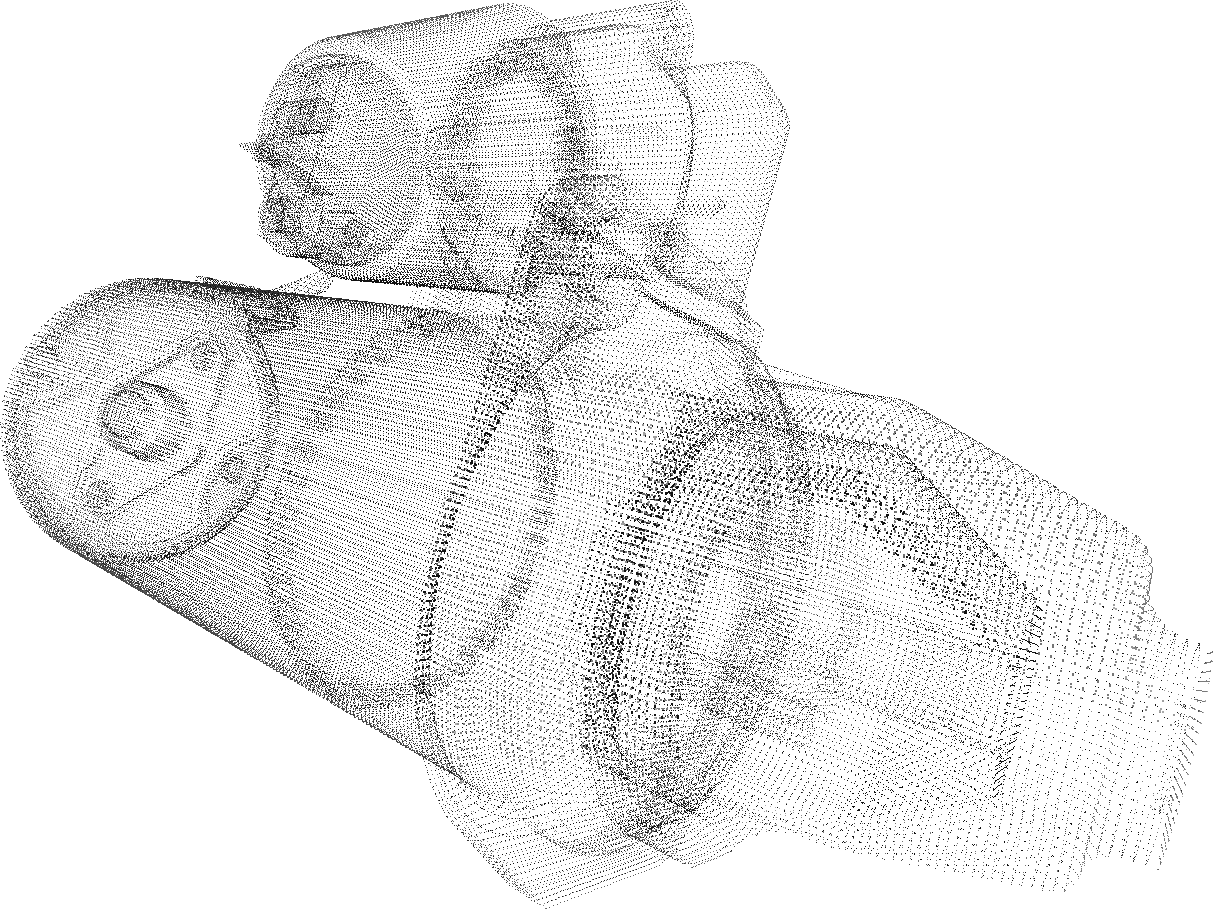
\includegraphics[height=.15\textheight]{sensor-data-processing/cad-model-pointcloud}
%	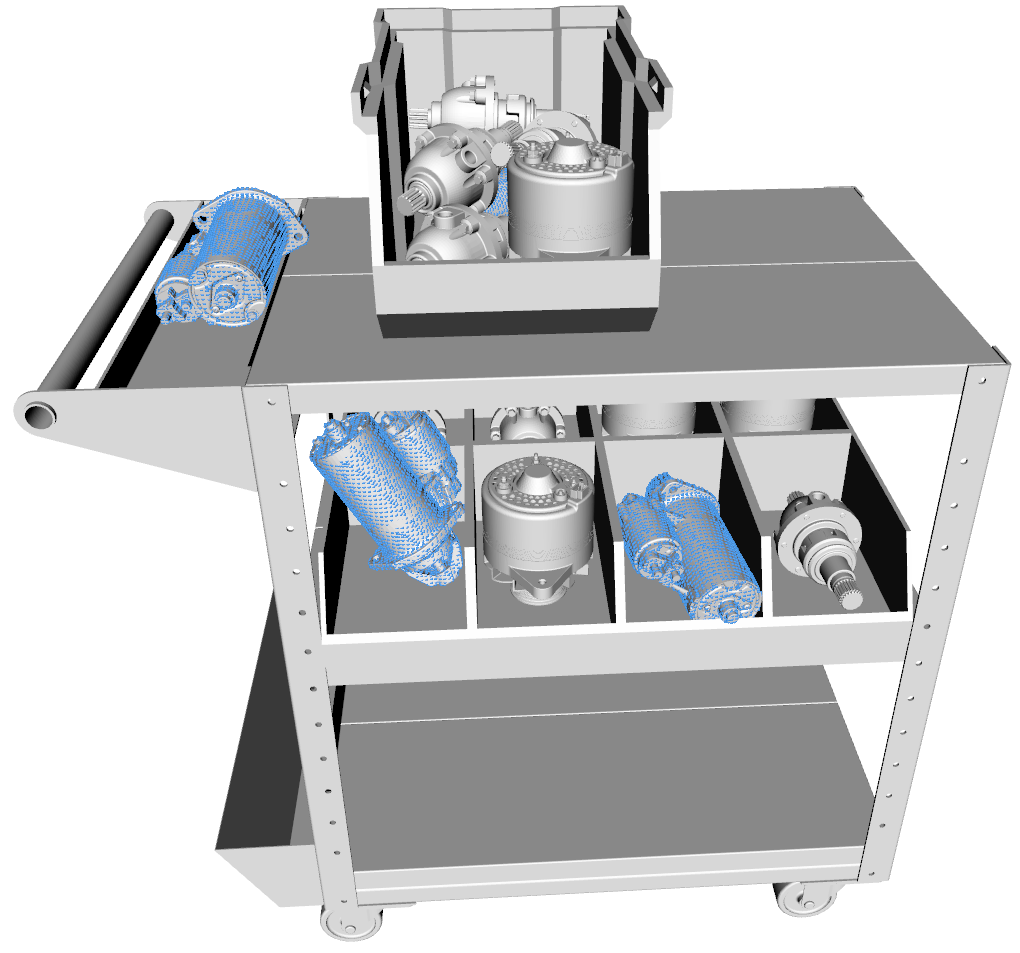
\includegraphics[height=.15\textheight]{sensor-data-processing/multimodel-pointclouds-with-cad}\hspace{2em}
	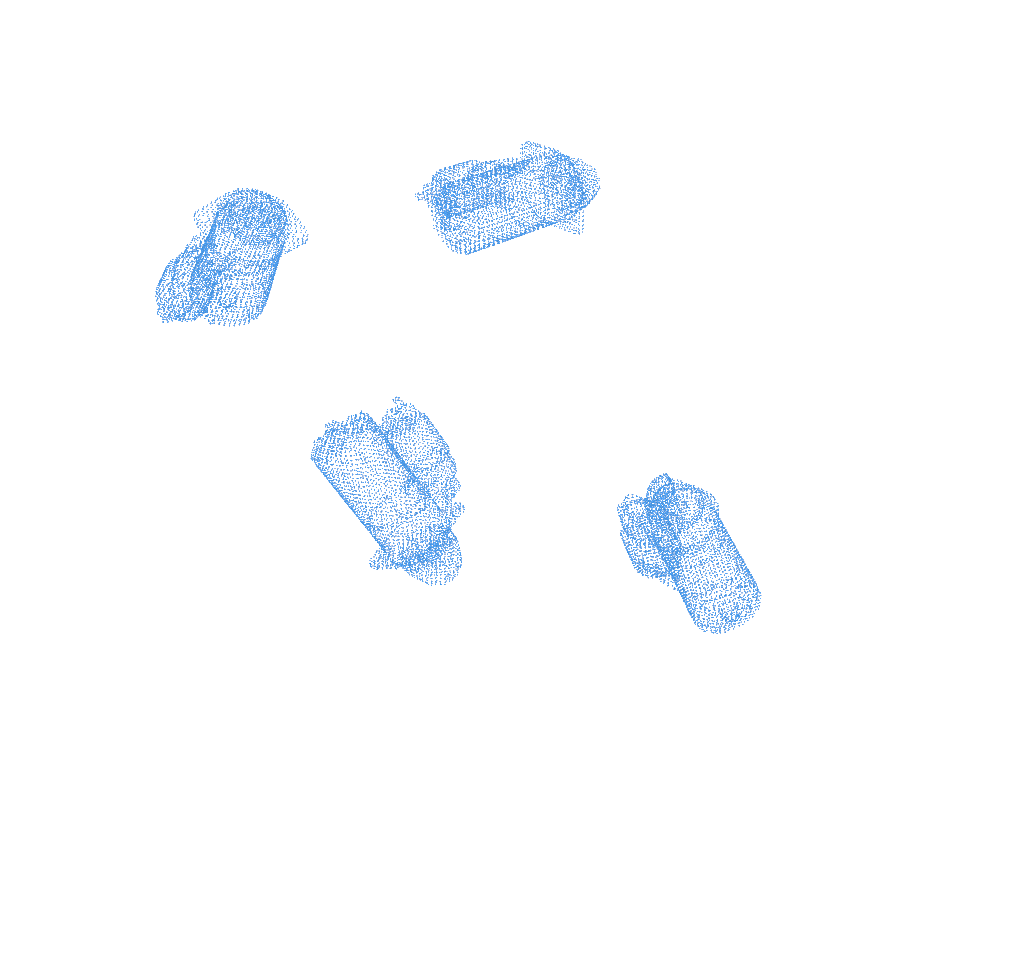
\includegraphics[height=.15\textheight]{sensor-data-processing/multimodel-pointclouds}
	\caption{Scene rendering from the Gazebo simulator with the 4 target objects in green color (left image) along with the associated reference point cloud that was generated for the 4 target objects (right image).}
	\label{fig:reference-cloud}
\end{figure}


\subsection{Sensors data analysis}

After loading the simulation world 3D models, deploying the sensors populations on the environment and building the filtered reference point cloud, the proposed system generates a color and depth image for every sensor. Then, for each pixel in the color images that have the target objects unique color (green), the corresponding pixel in the depth image is retrieved and using the pinhole model equations shown in \cref{eq:pointcloud}, the 3D point is computed from the 2D pixel coordinates and the depth value (retrieved form the OpenGL Z buffer). Later on, the 3D point is transformed from the sensor coordinate system into the world coordinate frame (having all sensor data in the same coordinate system allows fast merging of point clouds from several sensors).

After processing all pixels of a given color image, the associated point cloud in the world coordinate frame is filtered with a voxel grid algorithm with a cell size tuned for the objects geometry we are trying to observe (given that too many points on a small area of a large object do not provide a significant advantage for 3D perception and require more processing time). This allows to perform a regular space partition for extracting the centroid of each voxel containing sensor points. This step is critical for allowing consistent evaluation of the object(s) observed surface area percentage, given that sensors with different resolution or at varying distances may generate point clouds with different point density even when observing the same surface area. Moreover, given that both the reference point cloud and the sensor data point clouds were filtered in the same coordinate frame and with the same voxel grid cell size, the surface coverage percentage can be computed very efficiently by simply dividing the number of surface points in the filtered sensor data point cloud by the number of surface points in the filtered reference point cloud.

In the end of the sensor analysis stage (presented in \cref{alg:sensor-analysis}), each sensor is associated with a filtered point cloud in the world coordinate frame containing only points belonging to the target objects surface (example in \cref{fig:sensor-data-processing}).

\footnotesize
\begin{equation}\label{eq:pointcloud}
	\begin{split}
		X = \frac{(PixelColumn - XPrincipalPoint) \times PixelDepth}{XFocalLenght}\\
		Y = \frac{(PixelRow - YPrincipalPoint) \times PixelDepth}{YFocalLenght}\\
		Z = PixelDepth
	\end{split}
\end{equation}
\normalsize

\begin{algorithm}
	\caption{Sensor data analysis}
	\label{alg:sensor-analysis}
	\begin{algorithmic}[1]
		\State \textbf{Input:}
		\State $S \gets$ deployed sensors
		\State $C \gets$ target objects unique color
		\State $F \gets$ cell size for the voxel grid filter
		\Procedure{SensorAnalysis}{$S,C,F$}
			\State $q \gets Empty$\Comment{sensors filtered point clouds}
			\ForAll{s sensors in S}
				\State $c \gets RenderColorImage(s)$
				\State $d \gets RenderDepthImage(s)$
				\State $w \gets GetSensorWorldPose(s)$
				\State $u \gets Empty$\Comment{target objects points}
				\ForAll{y image rows in c}
					\ForAll{x image columns in c}
						\State $p \gets GetPixel(c,x,y)$
						\If{$p = C$}
							\State $k \gets GetDepth(d,x,y)$
							\If{$InValidRange(k,s)$}
								\State $j \gets 3DPoint(k,x,y,s)$
								\State $m \gets TransformPt(j,w)$
								\State $AppendPoint(u,m)$
							\EndIf
						\EndIf
					\EndFor
				\EndFor
				\State $z \gets FilterPointCloud(u,F)$
				\State $AppendPointCloud(q,z)$
			\EndFor
			\State \textbf{return} $(q)$
		\EndProcedure
	\end{algorithmic}
\end{algorithm}

\begin{figure}
	\centering
	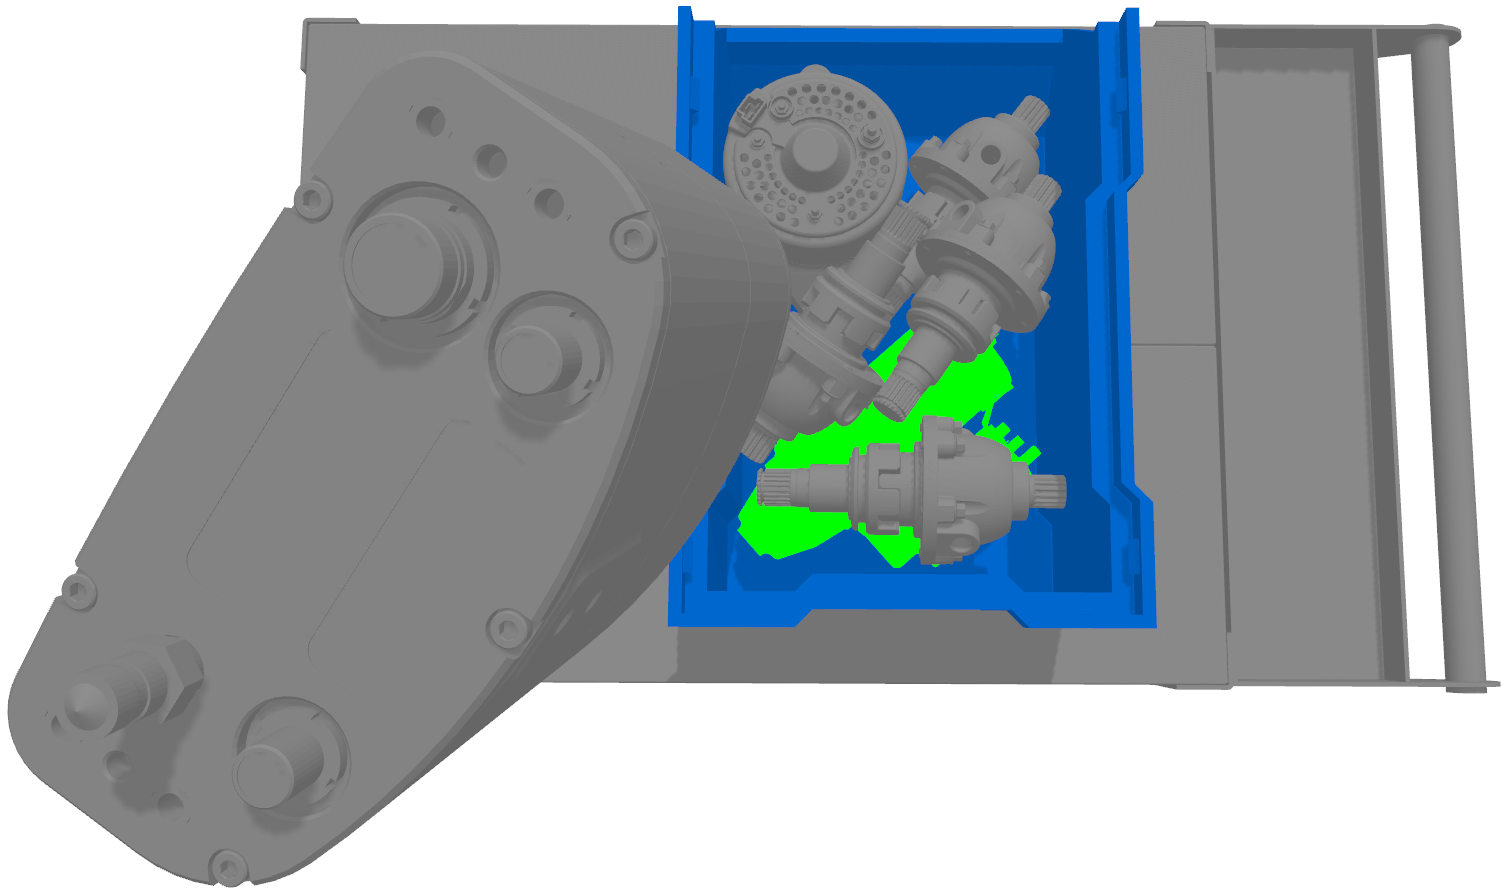
\includegraphics[height=.095\textheight]{sensor-data-processing/sensors-best-view}
	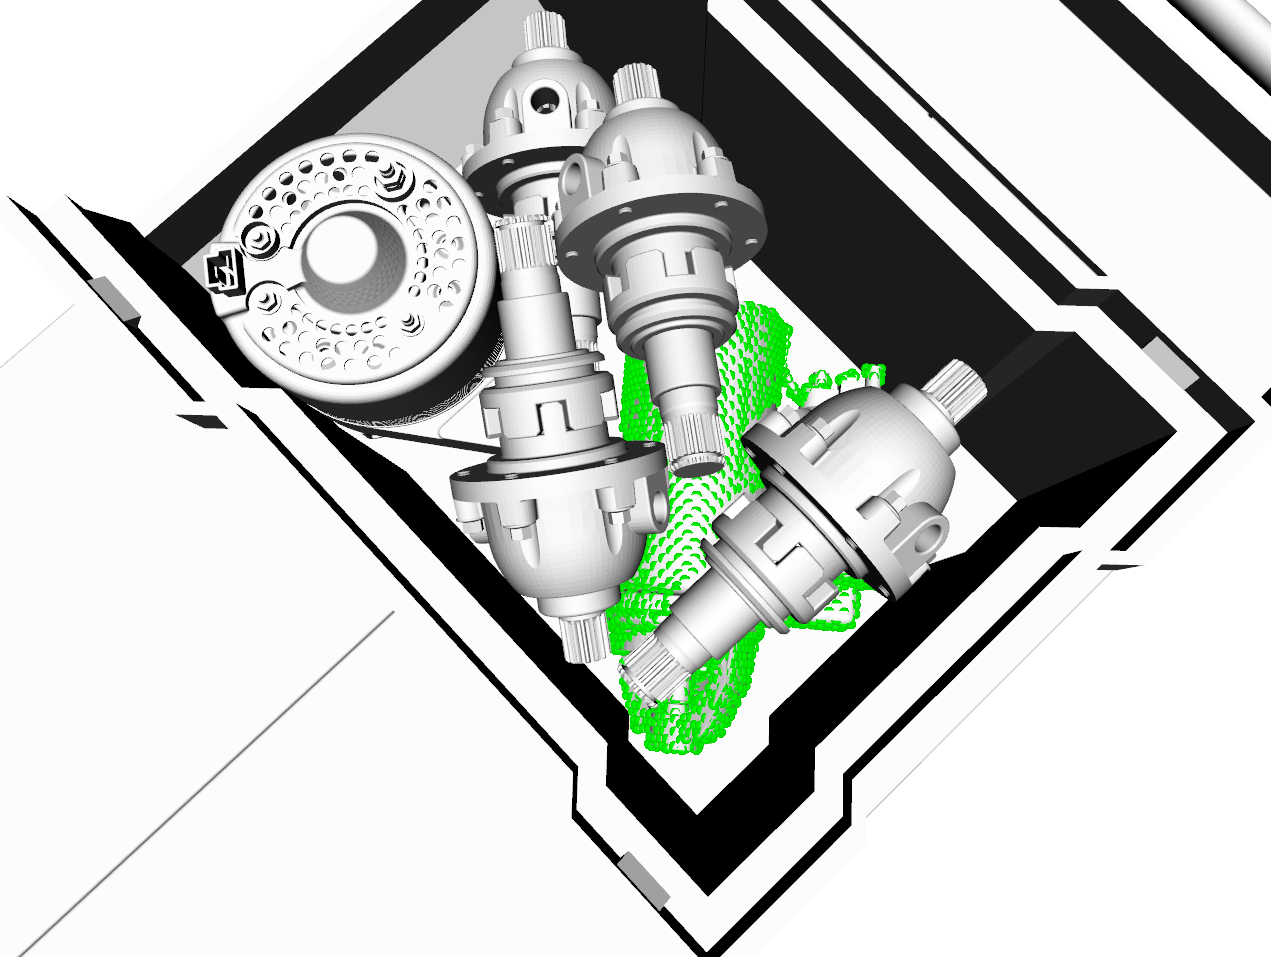
\includegraphics[height=.095\textheight]{sensor-data-processing/rviz-sensor-view}
	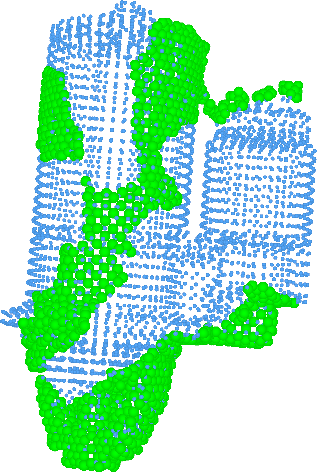
\includegraphics[height=.095\textheight]{sensor-data-processing/rviz-sensor-view-without-cad-with-model}
	\caption{Environment for bin picking of 1 object with occlusions along with the selected 3D sensor (left image) and with the generated point cloud for the target object taking into consideration the environment occlusions (center and right images, in which the green spheres are the points observed by the 3D sensor and the blue spheres are from the filtered reference point cloud).}
	\label{fig:sensor-data-processing}
\end{figure}


\subsection{Estimation of the best sensors views}

When only one sensor is needed for the task at hand (for example when we are trying to perform 3D perception of the environment in which the sensor is attached to a robotic arm), the estimation of the best sensor can be performed by simply selecting the one that achieved the best surface coverage area percentage. On the other hand, if several sensors are available or we want a single sensor to observe the target objects from a set of N best views, then it is used a \gls{ransac} approach to estimate the constellation of sensors that can achieve the best surface coverage. This approach allows to mitigate and bound the combinatorial explosion that happens when we need to estimate a high number of best views from a large population of sensors. As can be seen in \cref{alg:best-n-views}, this approach runs at most a fixed number of iterations. In each iteration, a set of N sensors are chosen randomly, their sensor data is merged and filtered, and if the surface coverage percentage achieved by this set of views is higher than a given threshold, then the search is stopped. In the end, it is returned the best sensor constellation found along with its associated point could (with the merged sensor data) and the best surface coverage percentage that was achieved.

\begin{algorithm}
	\caption{Estimation of the best N sensors views}
	\label{alg:best-n-views}
	\begin{algorithmic}[1]
		\State \textbf{Input:}
		\State $N \gets$ number of desired sensors
		\State $P \gets$ point clouds from each deployed sensor
		\State $F \gets$ cell size for the voxel grid filter
		\State $C \gets$ minimum surface coverage percentage
		\State $I \gets$ maximum number of iterations
		\Procedure{BestSensorsViews}{$N,P,F,C,I$}
			\State $s \gets Empty$\Comment{best coverage sensors}
			\State $p \gets Empty$\Comment{best merged point cloud}
			\State $c \gets 0$\Comment{best coverage percentage}
			\State $i \gets 0$\Comment{current iteration}
			\While{$i < I$ and $c < C$}
				\State $x \gets SelectSensorsRandomly(P,N)$
				\State $m \gets MergePointClouds(P,x)$
				\State $f \gets FilterPointCloud(m,F)$
				\State $k \gets ComputeSurfaceCoverage(f)$
				\State $i \gets i + 1$
				\If{$k > c$}
					\State $s \gets x$
					\State $p \gets f$
					\State $c \gets k$
				\EndIf
			\EndWhile
			\State \textbf{return} $(s,p,c)$
		\EndProcedure
	\end{algorithmic}
\end{algorithm}
